\documentclass[10pt,a4paper]{amsart}
\usepackage[margin=19mm]{geometry}
\usepackage{amsmath,amssymb,mathtools}
\usepackage[scr=rsfs,cal=euler]{mathalfa}
\usepackage{xfrac}
\usepackage[unicode,hidelinks,bookmarks=false]{hyperref}
\newcommand{\ie}{i.e.\ }
\newcommand{\cf}{cf.\ }
\newcommand{\resp}{respectively\ }
\newcommand{\Subsection}{\subsection}
\providecommand{\nobreakdash}{\nobreak\hbox{-}}
\setlength{\emergencystretch}{2em}
\multlinegap0pt
\usepackage{tikz}
\usepackage{amssymb}
\usepackage{xcolor}
\usepackage[normalem]{ulem}
\newtheorem{lemma}{Lemma}
\usepackage{cleveref}
\crefname{lemma}{Lemma}{Lemmas}
\title{The unknotting numbers for plus-welded knotoids}
\author{Fengling Li$^*$, Andrei Vesnin$^\dag$, Xuan Yang}
\date{Source: arXiv:2601.19549v1 (CC BY 4.0)}
\begin{document}
\maketitle

\noindent\emph{Source and licence.} The unknotting numbers for plus-welded knotoids. Version arXiv:2601.19549v1 (CC BY 4.0), distributed by arXiv under the Creative Commons Attribution 4.0 International licence, http://creativecommons.org/licenses/by/4.0/, as recorded in the arXiv licence metadata for this exact version and shown on the abstract page https://arxiv.org/abs/2601.19549v1. Full licence notice: \texttt{licenses/arxiv-2601.19549-CC-BY-4.0.txt}.\par\smallskip

\noindent\textit{Editorial scope.} Counted unit: the article's lemma 3.2 (source0.tex lines 782--784). The article's complete original proof of it is delivered with it (source0.tex lines 786--1078, one \texttt{proof} environment of 293 lines). No mathematics is written, repaired or re-derived: the statement and the proof are the article's own lines, in the article's own notation, and no retained line is substituted or re-flowed.  Retained uncounted as the source-local context the proof needs: lines 694--696.  Nothing was omitted from any retained span, so the package carries no omission record.  No retained line contains a citation, so the wrapper carries no bibliography and no bibliography entry.  The retained lines contain the article's own diagram code, which the wrapper typesets with the standard tikz packages; no image file is delivered and the package declares no asset dependency.  Editorial formatting only, in addition: an AMS \texttt{amsart} preamble that restates the article's own declarations and macros used by the retained lines, namely the environments \texttt{lemma} on separate counters, together with the standard packages those lines need.  The retained environments print in this document as Lemma 1 in order of appearance, whereas the article prints the same items with the numbering of its own full document.  The complete native source of the article as distributed in the arXiv e-print for this exact version is bundled unchanged as \texttt{sources/193462/source0.tex}.
\begin{lemma} \label{Lemma 3.1}
A Gauss diagram determines a virtual knotoid diagram up to virtual Reidemeister moves $V\Omega_1 - V\Omega_4$ and $\Omega_v$-move.  
\end{lemma}

\begin{lemma} \label{Lemma 3.2}	
Let $x$ be a classical crossing of a plus-welded knotoid diagram $D$. Consider two paths in which $D$ will split after smoothing at $x$. Suppose that one of the paths contains no under-crossing points other than $x$. Let $E$ be the plus-welded knotoid diagram obtained from $D$ by replacing $x$ with a welded crossing. Then, $D$ can be transformed into $E$ by a finite sequence of moves $\Omega_1$, $V\Omega_1 - V\Omega_4$, $\Omega_v$, $\Phi_{\text{over}}$, and $\Phi_+$. 
\end{lemma}

\begin{proof}
Let $\alpha$ be the path which has no under-crossing except $x$. Then $\alpha$ can be either a closed path or an open path. Since $x$ is the sole under-crossing on $\alpha$, the Gauss diagram corresponding to $\alpha$ includes only the starting points of the chords and does not contain the ending points of the chords other than $x$. Next, we will discuss it in two cases.

\underline{\textbf{Case 1.} $\alpha$ is a closed path.} We repeatedly apply $\Phi_{\text{over}}$-moves to contract the chord $c$ corresponding to $x$ into a trivial chord $c_1$, and then use one $\Omega_1$-move to eliminate $c_1$, thereby obtaining a new Gauss diagram $G(D')$. We find that $G(D') = G(E)$, and by~\cref{Lemma 3.1}, it follows that $D'$ can be transformed into $E$ under virtual Reidemeister moves $V\Omega_1 - V\Omega_4$ and $\Omega_v$-move. Consequently,
$D$ can be transformed into $E$ by a finite sequence of moves $\Omega_1$, $V\Omega_1 - V\Omega_4$, $\Omega_v$, and $\Phi_{\text{over}}$. The schematic diagram of this proof is shown in~\cref{Figure 14}. 
\begin{figure}[htbp]
\centering
\tikzset{every picture/.style={line width=1.5pt}}
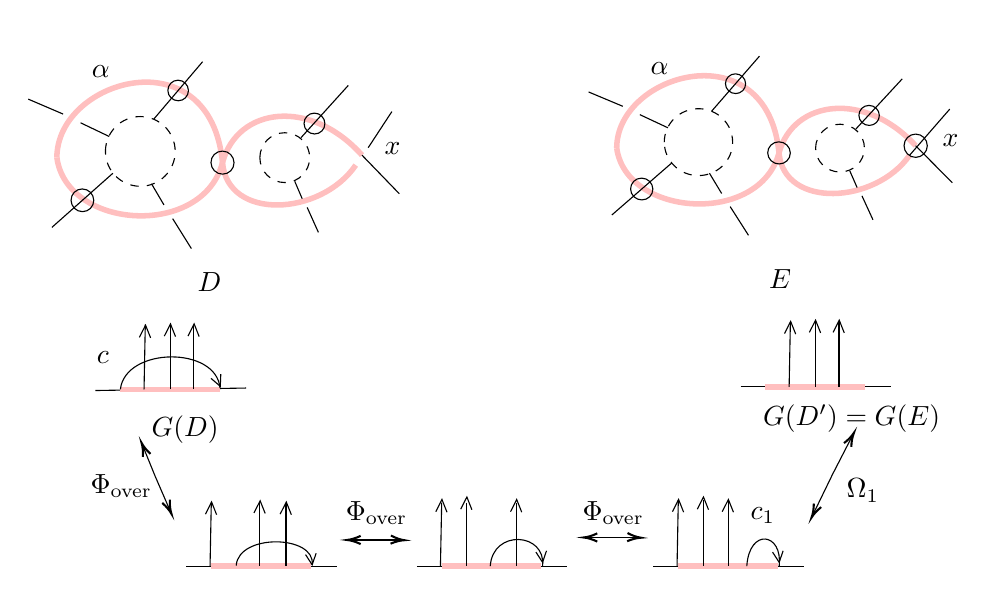
\begin{tikzpicture}[x=0.75pt,y=0.75pt,yscale=-0.6,xscale=0.6]
	\draw  [pink,line width=2pt]  (178,95) .. controls (190,50) and (249,43) .. (290,89) ;
	\draw  [pink,line width=2pt]   (45,91) .. controls (53,149) and (162,156) .. (178,95) ;
	\draw  [pink,line width=2pt]  (45,91) .. controls (45,28) and (168.07,-7.52) .. (178,95) ;
	\draw  [pink,line width=2pt]   (285,97) .. controls (257,138) and (182,142) .. (178,95) ;
	\draw    (295,83) -- (314,54) ;
	\draw    (241,75) -- (279,33) ;
	\draw    (121,112) -- (131,129) ;
	\draw    (290,89) -- (320,120) ;
	\draw    (122.76,60.13) -- (162,14) ;
	\draw    (64,63) -- (87,74) ;
	\draw    (153,164) -- (138,140) ;
	\draw   (243.47,63.63) .. controls (243.42,59) and (247.13,55.25) .. (251.76,55.25) .. controls (256.38,55.25) and (260.17,59) .. (260.22,63.63) .. controls (260.27,68.25) and (256.56,72) .. (251.94,72) .. controls (247.31,72) and (243.52,68.25) .. (243.47,63.63) -- cycle ;
	\draw   (56.38,125.25) .. controls (56.32,120.21) and (60.36,116.13) .. (65.4,116.13) .. controls (70.44,116.13) and (74.57,120.21) .. (74.62,125.25) .. controls (74.68,130.29) and (70.64,134.37) .. (65.6,134.37) .. controls (60.56,134.37) and (56.43,130.29) .. (56.38,125.25) -- cycle ;
	\draw   (134.12,37.07) .. controls (134.07,32.51) and (137.73,28.81) .. (142.29,28.81) .. controls (146.85,28.81) and (150.59,32.51) .. (150.64,37.07) .. controls (150.69,41.63) and (147.03,45.33) .. (142.47,45.33) .. controls (137.91,45.33) and (134.17,41.63) .. (134.12,37.07) -- cycle ;
	\draw   (168.74,95) .. controls (168.68,89.88) and (172.78,85.74) .. (177.9,85.74) .. controls (183.02,85.74) and (187.21,89.88) .. (187.26,95) .. controls (187.32,100.12) and (183.22,104.26) .. (178.1,104.26) .. controls (172.98,104.26) and (168.79,100.12) .. (168.74,95) -- cycle ;
	\draw [dashed]  (84,86) .. controls (84,70.54) and (96.54,58) .. (112,58) .. controls (127.46,58) and (140,70.54) .. (140,86) .. controls (140,101.46) and (127.46,114) .. (112,114) .. controls (96.54,114) and (84,101.46) .. (84,86) -- cycle ;
	\draw [dashed]  (208,91) .. controls (208,79.95) and (216.95,71) .. (228,71) .. controls (239.05,71) and (248,79.95) .. (248,91) .. controls (248,102.05) and (239.05,111) .. (228,111) .. controls (216.95,111) and (208,102.05) .. (208,91) -- cycle ;
	\draw    (50,56) -- (22,44) ;
	\draw    (242,124) -- (236,110) ;
	\draw    (246,131) -- (255,151) ;
	\draw    (90,103.5) -- (41,147) ;
	\draw [pink,line width=2pt]   (624.86,87.18) .. controls (636.62,44.03) and (694.43,37.31) .. (734.6,81.43) ;
	\draw  [pink,line width=2pt]  (494.54,83.35) .. controls (502.38,138.97) and (609.18,145.69) .. (624.86,87.18) ;
	\draw  [pink,line width=2pt]  (494.54,83.35) .. controls (494.54,22.93) and (615.13,-11.14) .. (624.86,87.18) ;
	\draw [pink,line width=2pt]   (729.7,89.1) .. controls (702.27,128.42) and (628.78,132.26) .. (624.86,87.18) ;
	\draw    (729.7,89.1) -- (762,52) ;
	\draw    (686.59,68) -- (723.83,27.72) ;
	\draw    (569.01,103.49) -- (578.81,119.79) ;
	\draw    (734.6,81.43) -- (764,111.16) ;
	\draw    (570.73,53.74) -- (609.18,9.5) ;
	\draw    (513.15,56.49) -- (535.69,67.04) ;
	\draw    (600.36,153.36) -- (585.66,130.34) ;
	\draw   (689.01,57.09) .. controls (688.97,52.66) and (692.6,49.06) .. (697.13,49.06) .. controls (701.67,49.06) and (705.38,52.66) .. (705.43,57.09) .. controls (705.48,61.53) and (701.84,65.13) .. (697.31,65.13) .. controls (692.78,65.13) and (689.06,61.53) .. (689.01,57.09) -- cycle ;
	\draw   (505.68,116.2) .. controls (505.63,111.36) and (509.59,107.44) .. (514.53,107.44) .. controls (519.47,107.44) and (523.51,111.36) .. (523.57,116.2) .. controls (523.62,121.03) and (519.66,124.95) .. (514.72,124.95) .. controls (509.78,124.95) and (505.74,121.03) .. (505.68,116.2) -- cycle ;
	\draw   (581.86,31.62) .. controls (581.82,27.25) and (585.4,23.7) .. (589.87,23.7) .. controls (594.34,23.7) and (598,27.25) .. (598.05,31.62) .. controls (598.1,36) and (594.51,39.54) .. (590.04,39.54) .. controls (585.57,39.54) and (581.91,36) .. (581.86,31.62) -- cycle ;
	\draw   (615.78,87.18) .. controls (615.73,82.28) and (619.75,78.3) .. (624.76,78.3) .. controls (629.77,78.3) and (633.88,82.28) .. (633.94,87.18) .. controls (633.99,92.09) and (629.97,96.07) .. (624.96,96.07) .. controls (619.94,96.07) and (615.84,92.09) .. (615.78,87.18) -- cycle ;
	\draw [dashed]  (532.75,78.55) .. controls (532.75,63.72) and (545.04,51.7) .. (560.19,51.7) .. controls (575.34,51.7) and (587.62,63.72) .. (587.62,78.55) .. controls (587.62,93.38) and (575.34,105.41) .. (560.19,105.41) .. controls (545.04,105.41) and (532.75,93.38) .. (532.75,78.55) -- cycle ;
	\draw [dashed]  (654.26,83.35) .. controls (654.26,72.75) and (663.03,64.17) .. (673.85,64.17) .. controls (684.68,64.17) and (693.45,72.75) .. (693.45,83.35) .. controls (693.45,93.94) and (684.68,102.53) .. (673.85,102.53) .. controls (663.03,102.53) and (654.26,93.94) .. (654.26,83.35) -- cycle ;
	\draw    (499.44,49.78) -- (472,38.27) ;
	\draw    (687.57,115) -- (681.69,101.57) ;
	\draw    (691.49,121.71) -- (700.31,140.89) ;
	\draw    (538.63,95.34) -- (490.62,137.06) ;
	\draw    (76,278) -- (197,276) ;
	\draw  [pink,line width=2pt]  (96,277) -- (176,277) ;
	\draw    (116,225) -- (115,277) ;
	\draw    (136,225) -- (136,277) ;
	\draw    (155,225) -- (155,277) ;
	\draw    (96,277) .. controls (100,243) and (173,242) .. (176,276) ;
	\draw   (176.62,264.84) -- (176.22,274.63) -- (168.79,268.25) ;
	\draw   (111.28,235.29) -- (116.22,225.51) -- (120.27,235.7) ;
	\draw   (131.28,234.29) -- (136.22,224.51) -- (140.27,234.7) ;
	\draw   (150.28,234.29) -- (155.22,224.51) -- (159.27,234.7) ;
	\draw    (149,419) -- (270,419) ;
	\draw  [pink,line width=2pt]    (169,419) -- (249,419) ;
	\draw    (169,368) -- (168,419) ;
	\draw    (229,368) -- (229,419) ;
	\draw    (208,368) -- (208,419) ;
	\draw    (189,418.5) .. controls (191,392.5) and (253,394) .. (250,418) ;
	\draw   (253.16,408.69) -- (250,417.96) -- (244.68,409.74) ;
	\draw   (164.28,377.29) -- (169.22,367.51) -- (173.27,377.7) ;
	\draw   (224.28,377.29) -- (229.22,367.51) -- (233.27,377.7) ;
	\draw   (203.28,376.29) -- (208.22,366.51) -- (212.27,376.7) ;
	\draw    (492,396) -- (512,396) ;
	\draw [shift={(514,396.2)}, rotate = 182.6] [color={rgb, 255:red, 0; green, 0; blue, 0 }  ][line width=0.75]    (10.93,-3.29) .. controls (6.95,-1.4) and (3.31,-0.3) .. (0,0) .. controls (3.31,0.3) and (6.95,1.4) .. (10.93,3.29)   ;
	\draw    (492,396) -- (470,396) ;
	\draw [shift={(468,396)}, rotate = 360] [color={rgb, 255:red, 0; green, 0; blue, 0 }  ][line width=0.75]    (10.93,-3.29) .. controls (6.95,-1.4) and (3.31,-0.3) .. (0,0) .. controls (3.31,0.3) and (6.95,1.4) .. (10.93,3.29)   ;
	\draw    (334,419) -- (455,419) ;
	\draw  [pink,line width=2pt]   (354,419) -- (434,419) ;
	\draw    (354,368) -- (353,419) ;	
	\draw    (414,368) -- (414,419) ;
	\draw    (374,368) -- (374,419) ;
	\draw    (393,419) .. controls (395,389) and (438,392) .. (435,419) ;
	\draw   (438.16,406.69) -- (435,415.96) -- (429.68,407.74) ;
	\draw   (349.28,375.29) -- (354.22,365.51) -- (358.27,375.7) ;
	\draw   (409.28,375.29) -- (414.22,365.51) -- (418.27,375.7) ;
	\draw   (369.28,373.29) -- (374.22,363.51) -- (378.27,373.7) ;
	\draw    (302,398) -- (322,398) ;
	\draw [shift={(324,398.2)}, rotate = 182.6] [color={rgb, 255:red, 0; green, 0; blue, 0 }  ][line width=0.75]    (10.93,-3.29) .. controls (6.95,-1.4) and (3.31,-0.3) .. (0,0) .. controls (3.31,0.3) and (6.95,1.4) .. (10.93,3.29)   ;
	\draw    (302,398) -- (280,398) ;
	\draw [shift={(278,398)}, rotate = 360] [color={rgb, 255:red, 0; green, 0; blue, 0 }  ][line width=0.75]    (10.93,-3.29) .. controls (6.95,-1.4) and (3.31,-0.3) .. (0,0) .. controls (3.31,0.3) and (6.95,1.4) .. (10.93,3.29)   ;		
	\draw    (524,419) -- (645,419) ;
	\draw  [pink,line width=2pt]   (544,419) -- (624,419) ;
	\draw    (544,366) -- (543,419) ;
	\draw    (584.5,366) -- (584.5,419) ;
	\draw    (564,366) -- (564,419) ;
	\draw    (599,419) .. controls (601,388) and (628,392) .. (625,419) ;
	\draw   (628.16,406.69) -- (625,415.96) -- (619.68,407.74) ;
	\draw   (539.28,375.29) -- (544.22,365.51) -- (548.27,375.7) ;
	\draw   (579.28,375.29) -- (584.22,365.51) -- (588.27,375.7) ;
	\draw   (559.28,373.29) -- (564.22,363.51) -- (568.27,373.7) ;
	\draw    (594,275) -- (715,275) ;
	\draw [pink,line width=2pt]    (614,275) -- (694,275) ;
	\draw    (634,223) -- (633,275) ;
	\draw    (654,223) -- (654,275) ;
	\draw    (673,223) -- (673,275) ;	
	\draw   (629.28,232.29) -- (634.22,222.51) -- (638.27,232.7) ;
	\draw   (649.28,231.29) -- (654.22,221.51) -- (658.27,231.7) ;
	\draw   (668.28,231.29) -- (673.22,221.51) -- (677.27,231.7) ;
	\draw    (124,347) -- (136.2,375.16) ;
	\draw [shift={(137,377)}, rotate = 246.57] [color={rgb, 255:red, 0; green, 0; blue, 0 }  ][line width=0.75]    (10.93,-3.29) .. controls (6.95,-1.4) and (3.31,-0.3) .. (0,0) .. controls (3.31,0.3) and (6.95,1.4) .. (10.93,3.29)   ;
	\draw    (124,347) -- (113.75,321.85) ;
	\draw [shift={(113,320)}, rotate = 67.83] [color={rgb, 255:red, 0; green, 0; blue, 0 }  ][line width=0.75]    (10.93,-3.29) .. controls (6.95,-1.4) and (3.31,-0.3) .. (0,0) .. controls (3.31,0.3) and (6.95,1.4) .. (10.93,3.29)   ;	
	\draw    (668,345) -- (684.08,313.78) ;
	\draw [shift={(685,312)}, rotate = 117.26] [color={rgb, 255:red, 0; green, 0; blue, 0 }  ][line width=0.75]    (10.93,-3.29) .. controls (6.95,-1.4) and (3.31,-0.3) .. (0,0) .. controls (3.31,0.3) and (6.95,1.4) .. (10.93,3.29)   ;
	\draw    (668,345) -- (651.87,378.2) ;
	\draw [shift={(651,380)}, rotate = 295.91] [color={rgb, 255:red, 0; green, 0; blue, 0 }  ][line width=0.75]    (10.93,-3.29) .. controls (6.95,-1.4) and (3.31,-0.3) .. (0,0) .. controls (3.31,0.3) and (6.95,1.4) .. (10.93,3.29)   ;
	\draw   (725.27,81.43) .. controls (725.27,76.27) and (729.45,72.09) .. (734.6,72.09) .. controls (739.76,72.09) and (743.94,76.27) .. (743.94,81.43) .. controls (743.94,86.59) and (739.76,90.77) .. (734.6,90.77) .. controls (729.45,90.77) and (725.27,86.59) .. (725.27,81.43) -- cycle ;
	% Text Node
	\draw (71,15) node [anchor=north west][inner sep=0.75pt]   [align=left] {$\alpha$};
	\draw (156,181.5) node [anchor=north west][inner sep=0.75pt]   [align=left] {$D$};
	\draw (306,77) node [anchor=north west][inner sep=0.75pt]   [align=left] {$x$};
	\draw (519.75,12.51) node [anchor=north west][inner sep=0.75pt]   [align=left] {$\alpha$};
	\draw (614.83,179.08) node [anchor=north west][inner sep=0.75pt]   [align=left] {$E$};
	\draw (754.17,70.57) node [anchor=north west][inner sep=0.75pt]   [align=left] {$x$};
	\draw (119,296) node [anchor=north west][inner sep=0.75pt]   [align=left] {$G(D)$};
	\draw (275,365) node [anchor=north west][inner sep=0.75pt]   [align=left] {$\Phi_{\text{over}}$};
	\draw (465,365) node [anchor=north west][inner sep=0.75pt]   [align=left] {$\Phi_{\text{over}}$};
	\draw (610,287) node [anchor=north west][inner sep=0.75pt]   [align=left] {$G(D')=G(E)$};
	\draw (70,343) node [anchor=north west][inner sep=0.75pt]   [align=left] {$\Phi_{\text{over}}$};
	\draw (677,347) node [anchor=north west][inner sep=0.75pt]   [align=left] {$\Omega_{1}$};
	\draw (75,245) node [anchor=north west][inner sep=0.75pt]   [align=left] {$c$};
	\draw (600,370) node [anchor=north west][inner sep=0.75pt]   [align=left] {$c_1$};
	
\end{tikzpicture}
\caption{A schematic diagram when $\alpha$ is a closed path.}
\label{Figure 14}
\end{figure}

\underline{\textbf{Case 2.} $\alpha$ is an open path.}  
Firstly, we repeatedly apply $\Phi_{\text{over}}$-moves to contract the chord $c$ corresponding to $x$ into a chord $c_1$, where the starting point of $c_1$ is the first starting point encountered when departing from any endpoint of the Gauss diagram. 
Subsequently, we utilize one $\Phi_+$-move to eliminate $c_1$, thus obtaining a new Gauss diagram $G(D')$.
It can be observed that $G(D') = G(E)$. By virtue of~\cref{Lemma 3.1}, $D'$ can be transformed into $E$ under virtual Reidemeister moves $V\Omega_1 - V\Omega_4$ and $\Omega_v$-moves. Therefore, $D$ can be transformed into $E$ through a finite sequence of moves $\Omega_{1}$, $V\Omega_1 - V\Omega_4$, $\Omega_v$, $\Phi_{\text{over}}$, and $\Phi_+$. The schematic diagram of this proof is shown in~\cref{Figure 15}. 
\begin{figure}[htbp]
\centering
\tikzset{every picture/.style={line width=1.5pt}} %set default line width to 0.75pt
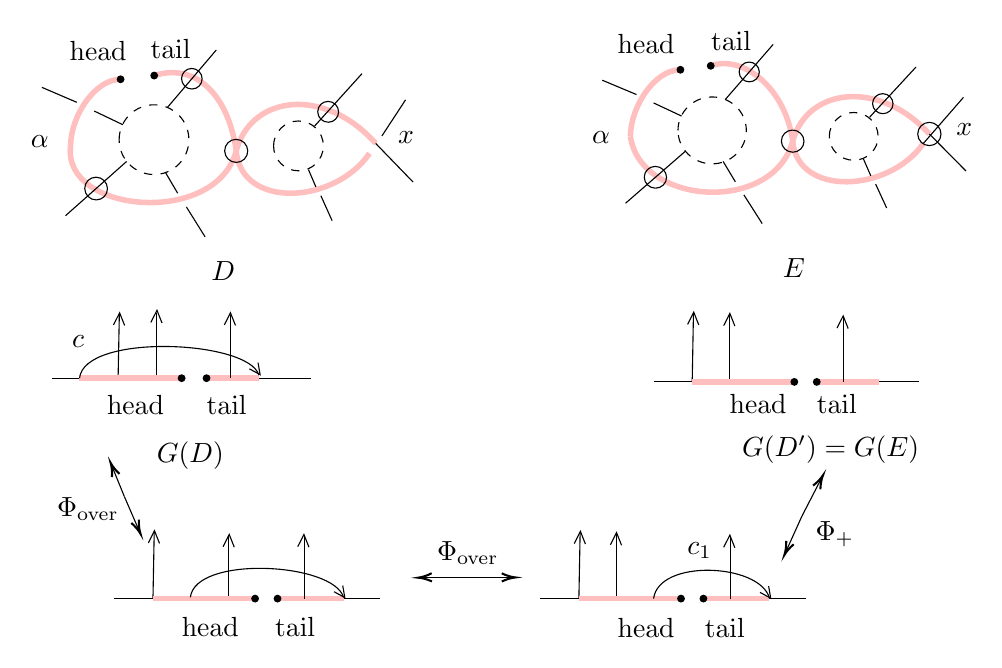
\begin{tikzpicture}[x=0.75pt,y=0.75pt,yscale=-0.6,xscale=0.6]
	\draw [pink,line width=2pt]  (175.83,98.49) .. controls (187.83,53.49) and (246.83,46.49) .. (287.83,92.49) ;
	\draw [pink,line width=2pt]   (42.83,94.49) .. controls (36,149) and (159.83,159.49) .. (175.83,98.49) ;
	\draw  [pink,line width=2pt]   (282.83,100.49) .. controls (254.83,141.49) and (179.83,145.49) .. (175.83,98.49) ;
	\draw  [pink,line width=2pt] (42.83,94.49) .. controls (43,71) and (62,41) .. (83,41) ;
	\draw  [pink,line width=2pt]  (110,38) .. controls (145,27) and (170,56) .. (175.83,98.49) ;
    \filldraw[color={rgb, 255:red, 0; green, 0; blue, 0 }  ,draw opacity=1] (83,41) circle (2pt);
	\filldraw[color={rgb, 255:red, 0; green, 0; blue, 0 }  ,draw opacity=1] (110,38) circle (2pt);
	\draw    (292.83,86.49) -- (311.83,57.49) ;
	\draw    (238.83,78.49) -- (276.83,36.49) ;
	\draw    (118.83,115.49) -- (128.83,132.49) ;
	\draw    (287.83,92.49) -- (317.83,123.49) ;
	\draw    (120.59,63.62) -- (159.83,17.49) ;
	\draw    (61.83,66.49) -- (84.83,77.49) ;
	\draw    (150.83,167.49) -- (135.83,143.49) ;
	\draw   (241.3,67.12) .. controls (241.25,62.49) and (244.96,58.74) .. (249.59,58.74) .. controls (254.21,58.74) and (258,62.49) .. (258.05,67.12) .. controls (258.1,71.74) and (254.39,75.49) .. (249.77,75.49) .. controls (245.14,75.49) and (241.35,71.74) .. (241.3,67.12) -- cycle ;
	\draw   (54.2,128.74) .. controls (54.15,123.7) and (58.19,119.62) .. (63.23,119.62) .. controls (68.27,119.62) and (72.4,123.7) .. (72.45,128.74) .. controls (72.51,133.78) and (68.47,137.87) .. (63.43,137.87) .. controls (58.39,137.87) and (54.26,133.78) .. (54.2,128.74) -- cycle ;
	\draw   (131.95,40.56) .. controls (131.9,36) and (135.56,32.3) .. (140.12,32.3) .. controls (144.68,32.3) and (148.42,36) .. (148.47,40.56) .. controls (148.52,45.12) and (144.86,48.82) .. (140.3,48.82) .. controls (135.74,48.82) and (132,45.12) .. (131.95,40.56) -- cycle ;
	\draw   (166.57,98.49) .. controls (166.51,93.38) and (170.61,89.23) .. (175.73,89.23) .. controls (180.84,89.23) and (185.04,93.38) .. (185.09,98.49) .. controls (185.15,103.61) and (181.04,107.75) .. (175.93,107.75) .. controls (170.81,107.75) and (166.62,103.61) .. (166.57,98.49) -- cycle ;
	\draw [dashed]  (81.83,89.49) .. controls (81.83,74.03) and (94.36,61.49) .. (109.83,61.49) .. controls (125.29,61.49) and (137.83,74.03) .. (137.83,89.49) .. controls (137.83,104.96) and (125.29,117.49) .. (109.83,117.49) .. controls (94.36,117.49) and (81.83,104.96) .. (81.83,89.49) -- cycle ;
	\draw [dashed]  (205.83,94.49) .. controls (205.83,83.45) and (214.78,74.49) .. (225.83,74.49) .. controls (236.87,74.49) and (245.83,83.45) .. (245.83,94.49) .. controls (245.83,105.54) and (236.87,114.49) .. (225.83,114.49) .. controls (214.78,114.49) and (205.83,105.54) .. (205.83,94.49) -- cycle ;
	\draw    (47.83,59.49) -- (19.83,47.49) ;
	\draw    (239.83,127.49) -- (233.83,113.49) ;
	\draw    (243.83,134.49) -- (252.83,154.49) ;
	\draw    (87.83,106.99) -- (38.83,150.49) ;
	\draw  [pink,line width=2pt]   (622.69,90.68) .. controls (634.45,47.52) and (692.26,40.8) .. (732.43,84.92) ;
	\draw  [pink,line width=2pt]   (492.37,86.84) .. controls (500.2,142.46) and (607.01,149.18) .. (622.69,90.68) ;
	\draw  [pink,line width=2pt]  (727.53,92.59) .. controls (700.1,131.92) and (626.61,135.75) .. (622.69,90.68) ;
	\draw [pink,line width=2pt]   (556.86,30.18) .. controls (583,21) and (616.86,48.18) .. (622.69,90.68) ;
	\draw  [pink,line width=2pt]  (492.37,86.84) .. controls (492.54,63.35) and (511.54,33.35) .. (532.54,33.35) ;
	\filldraw[color={rgb, 255:red, 0; green, 0; blue, 0 }  ,draw opacity=1] (532.54,33.35) circle (2pt);
	\filldraw[color={rgb, 255:red, 0; green, 0; blue, 0 }  ,draw opacity=1] (556.86,30.18) circle (2pt);
	\draw    (727.53,92.59) -- (759.83,55.49) ;
	\draw    (684.42,71.49) -- (721.65,31.21) ;
	\draw    (566.84,106.98) -- (576.63,123.28) ;
	\draw    (732.43,84.92) -- (761.83,114.65) ;
	\draw    (568.56,57.24) -- (607.01,12.99) ;
	\draw    (510.98,59.99) -- (533.52,70.54) ;
	\draw    (598.19,156.85) -- (583.49,133.83) ;
	\draw   (686.84,60.58) .. controls (686.79,56.15) and (690.43,52.55) .. (694.96,52.55) .. controls (699.49,52.55) and (703.21,56.15) .. (703.26,60.58) .. controls (703.31,65.02) and (699.67,68.62) .. (695.14,68.62) .. controls (690.61,68.62) and (686.89,65.02) .. (686.84,60.58) -- cycle ;
	\draw   (503.51,119.69) .. controls (503.46,114.85) and (507.42,110.94) .. (512.36,110.94) .. controls (517.29,110.94) and (521.34,114.85) .. (521.39,119.69) .. controls (521.45,124.52) and (517.49,128.44) .. (512.55,128.44) .. controls (507.61,128.44) and (503.56,124.52) .. (503.51,119.69) -- cycle ;
	\draw   (579.69,35.11) .. controls (579.64,30.74) and (583.23,27.19) .. (587.7,27.19) .. controls (592.17,27.19) and (595.83,30.74) .. (595.88,35.11) .. controls (595.93,39.49) and (592.34,43.03) .. (587.87,43.03) .. controls (583.4,43.03) and (579.74,39.49) .. (579.69,35.11) -- cycle ;
	\draw   (613.61,90.68) .. controls (613.56,85.77) and (617.58,81.79) .. (622.59,81.79) .. controls (627.6,81.79) and (631.71,85.77) .. (631.76,90.68) .. controls (631.82,95.58) and (627.8,99.56) .. (622.79,99.56) .. controls (617.77,99.56) and (613.67,95.58) .. (613.61,90.68) -- cycle ;
	\draw [dashed]  (530.58,82.04) .. controls (530.58,67.21) and (542.86,55.19) .. (558.02,55.19) .. controls (573.17,55.19) and (585.45,67.21) .. (585.45,82.04) .. controls (585.45,96.87) and (573.17,108.9) .. (558.02,108.9) .. controls (542.86,108.9) and (530.58,96.87) .. (530.58,82.04) -- cycle ;
	\draw [dashed]  (652.08,86.84) .. controls (652.08,76.25) and (660.86,67.66) .. (671.68,67.66) .. controls (682.5,67.66) and (691.28,76.25) .. (691.28,86.84) .. controls (691.28,97.43) and (682.5,106.02) .. (671.68,106.02) .. controls (660.86,106.02) and (652.08,97.43) .. (652.08,86.84) -- cycle ;
	\draw    (497.27,53.27) -- (469.83,41.76) ;
	\draw    (685.4,118.49) -- (679.52,105.06) ;
	\draw    (689.32,125.2) -- (698.14,144.38) ;
	\draw    (536.46,98.83) -- (488.45,140.55) ;
	\draw   (723.1,84.92) .. controls (723.1,79.76) and (727.28,75.58) .. (732.43,75.58) .. controls (737.59,75.58) and (741.77,79.76) .. (741.77,84.92) .. controls (741.77,90.08) and (737.59,94.26) .. (732.43,94.26) .. controls (727.28,94.26) and (723.1,90.08) .. (723.1,84.92) -- cycle ;
	\draw    (152,281) -- (236,281) ;
	\draw  [pink,line width=2pt]  (152,281) -- (194,281) ;
	\draw    (82,229) -- (81,281) ;
	\draw    (112,229) -- (112,281) ;
	\draw    (171,230) -- (171,281) ;
	\draw    (28,281) -- (132,281) ;
	\draw  [pink,line width=2pt]   (50,281) -- (132,281) ;
	\filldraw[color={rgb, 255:red, 0; green, 0; blue, 0 }  ,draw opacity=1] (132,281) circle (2pt);
	\filldraw[color={rgb, 255:red, 0; green, 0; blue, 0 }  ,draw opacity=1] (152,281) circle (2pt);
	\draw    (50,281) .. controls (54,244.5) and (186,250.5) .. (194,278.5) ;
	\draw   (193.36,268.52) -- (195.03,278.17) -- (186.42,273.49) ;
	\draw   (77.28,238.29) -- (82.22,228.51) -- (86.27,238.7) ;
	\draw   (107.28,236.29) -- (112.22,226.51) -- (116.27,236.7) ;
	\draw   (166.28,238.29) -- (171.22,228.51) -- (175.27,238.7) ;
	\draw    (209,458) -- (291,458) ;
	\draw [pink,line width=2pt]  (209,458) -- (262,458) ;
	\draw    (110,404.5) -- (109,458) ;
	\draw    (170,407) -- (170,458) ;
	\draw    (78,458) -- (191,458) ;
	\draw  [pink,line width=2pt]   (109,458) -- (191,458) ;
	\draw   (230.5,407.75) -- (230.5,458) ;
	\filldraw[color={rgb, 255:red, 0; green, 0; blue, 0 }  ,draw opacity=1] (191,458) circle (2pt);
	\filldraw[color={rgb, 255:red, 0; green, 0; blue, 0 }  ,draw opacity=1] (209,458) circle (2pt);
	\draw    (139,457) .. controls (143,423) and (254,429) .. (262,457) ;
	\draw   (261.36,447.52) -- (263.03,457.17) -- (254.42,452.49) ;
	\draw   (105.28,413.29) -- (110.22,403.51) -- (114.27,413.7) ;
	\draw   (165.28,416.29) -- (170.22,406.51) -- (174.27,416.7) ;
	\draw   (225.28,416.29) -- (230.22,406.51) -- (234.27,416.7) ;
	\draw    (551,458) -- (633,458) ;
	\draw [pink,line width=2pt]    (551,458) -- (604,458) ;
	\draw    (452,405) -- (451,458) ;
	\draw    (481,406) -- (481,458) ;
	\draw    (572.5,408.25) -- (572.5,458) ;
	\draw    (420,458) -- (533,458) ;
	\draw  [pink,line width=2pt]   (451,458) -- (533,458) ;
	\filldraw[color={rgb, 255:red, 0; green, 0; blue, 0 }  ,draw opacity=1] (551,458) circle (2pt);
	\filldraw[color={rgb, 255:red, 0; green, 0; blue, 0 }  ,draw opacity=1] (533,458) circle (2pt);
	\draw    (511,458) .. controls (515,426) and (596,429.5) .. (604,457.5) ;
	\draw   (603.36,448.02) -- (605.03,457.67) -- (596.42,452.99) ;
	\draw   (447.28,413.79) -- (452.22,404.01) -- (456.27,414.2) ;
	\draw   (476.28,414.79) -- (481.22,405.01) -- (485.27,415.2) ;
	\draw   (567.28,416.79) -- (572.22,407.01) -- (576.27,417.2) ;
	\draw    (642,284) -- (724,284) ;
	\draw  [pink,line width=2pt]  (642,284) -- (692,284) ;
	\draw    (543,229) -- (542,284) ;
	\draw    (572,230) -- (572,284) ;
	\draw    (511,284) -- (624,284) ;
	\draw [pink,line width=2pt]   (542,284) -- (624,284) ;
	\draw    (663.5,232.25) -- (663.5,284) ;
	\filldraw[color={rgb, 255:red, 0; green, 0; blue, 0 }  ,draw opacity=1] (624,284) circle (2pt);
	\filldraw[color={rgb, 255:red, 0; green, 0; blue, 0 }  ,draw opacity=1] (642,284) circle (2pt);
	\draw   (538.28,237.79) -- (543.22,228.01) -- (547.27,238.2) ;
	\draw   (567.28,238.79) -- (572.22,229.01) -- (576.27,239.2) ;
	\draw   (658.28,240.79) -- (663.22,231.01) -- (667.27,241.2) ;
	\draw    (86,376) -- (98.2,404.16) ;
	\draw [shift={(99,406)}, rotate = 246.57] [color={rgb, 255:red, 0; green, 0; blue, 0 }  ][line width=0.75]    (10.93,-3.29) .. controls (6.95,-1.4) and (3.31,-0.3) .. (0,0) .. controls (3.31,0.3) and (6.95,1.4) .. (10.93,3.29)   ;
	\draw    (86,376) -- (75.75,350.85) ;
	\draw [shift={(75,349)}, rotate = 67.83] [color={rgb, 255:red, 0; green, 0; blue, 0 }  ][line width=0.75]    (10.93,-3.29) .. controls (6.95,-1.4) and (3.31,-0.3) .. (0,0) .. controls (3.31,0.3) and (6.95,1.4) .. (10.93,3.29)   ;
	\draw    (630,392) -- (646.08,360.78) ;
	\draw [shift={(647,359)}, rotate = 117.26] [color={rgb, 255:red, 0; green, 0; blue, 0 }  ][line width=0.75]    (10.93,-3.29) .. controls (6.95,-1.4) and (3.31,-0.3) .. (0,0) .. controls (3.31,0.3) and (6.95,1.4) .. (10.93,3.29)   ;
	\draw    (630,392) -- (616.82,421.18) ;
	\draw [shift={(616,423)}, rotate = 294.3] [color={rgb, 255:red, 0; green, 0; blue, 0 }  ][line width=0.75]    (10.93,-3.29) .. controls (6.95,-1.4) and (3.31,-0.3) .. (0,0) .. controls (3.31,0.3) and (6.95,1.4) .. (10.93,3.29)   ;
	\draw    (360,441) -- (398,441) ;
	\draw [shift={(400,441)}, rotate = 180] [color={rgb, 255:red, 0; green, 0; blue, 0 }  ][line width=0.75]    (10.93,-3.29) .. controls (6.95,-1.4) and (3.31,-0.3) .. (0,0) .. controls (3.31,0.3) and (6.95,1.4) .. (10.93,3.29)   ;
	\draw    (360,441) -- (324,441) ;
	\draw [shift={(322,441.2)}, rotate = 358.49] [color={rgb, 255:red, 0; green, 0; blue, 0 }  ][line width=0.75]    (10.93,-3.29) .. controls (6.95,-1.4) and (3.31,-0.3) .. (0,0) .. controls (3.31,0.3) and (6.95,1.4) .. (10.93,3.29)   ;
	% Text Node
	\draw (8.83,83.99) node [anchor=north west][inner sep=0.75pt]   [align=left] {$\alpha$};
	\draw (153.83,184.99) node [anchor=north west][inner sep=0.75pt]   [align=left] {$D$};
	\draw (303.83,80.49) node [anchor=north west][inner sep=0.75pt]   [align=left] {$x$};
	\draw (459.58,81) node [anchor=north west][inner sep=0.75pt]   [align=left] {$\alpha$};
	\draw (612.66,182.57) node [anchor=north west][inner sep=0.75pt]   [align=left] {$E$};
	\draw (752,74.06) node [anchor=north west][inner sep=0.75pt]   [align=left] {$x$};
	\draw (110,330) node [anchor=north west][inner sep=0.75pt]   [align=left] {$G(D)$};
	\draw (580,325) node [anchor=north west][inner sep=0.75pt]   [align=left] {$G(D')=G(E)$};
	\draw (70,292.5) node [anchor=north west][inner sep=0.75pt]   [align=left] {head};
	\draw (150,292.5) node [anchor=north west][inner sep=0.75pt]   [align=left] {tail};
	\draw (130,470.5) node [anchor=north west][inner sep=0.75pt]   [align=left] {head};
	\draw (205,470.5) node [anchor=north west][inner sep=0.75pt]   [align=left] {tail};
	\draw (480,472) node [anchor=north west][inner sep=0.75pt]   [align=left] {head};
	\draw (550,472) node [anchor=north west][inner sep=0.75pt]   [align=left] {tail};
	\draw (570,292) node [anchor=north west][inner sep=0.75pt]   [align=left] {head};
	\draw (640,292) node [anchor=north west][inner sep=0.75pt]   [align=left] {tail};	
	\draw (40,8) node [anchor=north west][inner sep=0.75pt]   [align=left] {head};
	\draw (105,7) node [anchor=north west][inner sep=0.75pt]   [align=left] {tail};
	\draw (480,3) node [anchor=north west][inner sep=0.75pt]   [align=left] {head};
	\draw (555,0) node [anchor=north west][inner sep=0.75pt]   [align=left] {tail};
	\draw (30,375) node [anchor=north west][inner sep=0.75pt]   [align=left] {$\Phi_{\text{over}}$};
	\draw (639,394) node [anchor=north west][inner sep=0.75pt]   [align=left] {$\Phi_+$};
	\draw (335,410) node [anchor=north west][inner sep=0.75pt]   [align=left] {$\Phi_{\text{over}}$};
	\draw (42,245) node [anchor=north west][inner sep=0.75pt]   [align=left] {$c$};
	\draw (536,411) node [anchor=north west][inner sep=0.75pt]   [align=left] {$c_1$};
\end{tikzpicture}
\caption{A schematic diagram when $\alpha$ is an open path.}
\label{Figure 15}
\end{figure}

This completes the proof of \cref{Lemma 3.2}.
\end{proof}

\end{document}
